\documentclass{article}


% Formatting
\usepackage[utf8]{inputenc}
\usepackage[margin=1in]{geometry}
\usepackage[titletoc,title]{appendix}
\usepackage{setspace}
\setlength{\parindent}{0 cm}

% Math
\usepackage{amsmath,amsfonts,amssymb,mathtools}
\usepackage{upquote}

% Images
\usepackage{graphicx,float}

% Tables
\usepackage[ruled,vlined]{algorithm2e}
\usepackage{algorithmic}

% Code syntax highlighting
\usepackage{minted}
\usemintedstyle{borland}


% Title content
\title{ECON302 Midterm}
\author{2219806 - Merve Öğretmek \\
2219897 - İpek Sanrı}

\linespread{1.25}
\begin{document}

\maketitle

\Large
\underline{\textbf{Part A}}
\small

\setcounter{section}{1}

\section{}

\textbf{a.}

\begin{equation}
    y_t = \rho y_{t-1} + u_t  
\end{equation}

where $u_t$ is normally and independently distributed with mean 0 and variance $1-\rho^2$
\\

First, we should note that variance of $u_t$ is equal to $1-\rho^2$ and since it is a variance, it has to be positive by definition.

\begin{align}
    \begin{split}
        1 - \rho^2 \geq 0 \ \ =>\ \ 1 \geq \rho^2 \ \ =>\ \ |\rho| < 1
    \end{split}
\end{align}

which indicates that impact decreases over time.
\\

\underline{Mean of $y_t$:}

We can write 

\begin{align}
    \begin{split}
        y_{t-1} = \rho y_{t-2} + u_{t-1} \\
        y_{t-2} = \rho y_{t-3} + u_{t-2} \\
        ...
    \end{split}
\end{align} 

an so on. by substituting y variables in each other, we end up with

\begin{align}
    \begin{split}
         y_t = u_t + \rho u_{t-1} + \rho^2 u_{t-2} + \rho^3  u_{t-3} + ... = \sum_{i=0}^\infty \rho^{i} u_{t-i}
    \end{split}
\end{align}

Now, we can take the expectation of $y_t$,

\begin{equation}
    E(y_t) = \sum_{i=0}^\infty \rho^{i} E(u_{t-i}) = 0
\end{equation}

In the question, it is given that $E(u_t)$  is normally independently distributed with mean 0. Therefore, putting the 0 in above equation for $E(u_{t-i})$ yields that mean of $y_t$ is also equal to 0.
\\

\underline{Variance of $y_t$:}

\begin{equation}
    Var(y_t) = Var(\rho y_{t-1} + u_t) = \rho^2 Var(y_{t-1}) + Var(u_t)
\end{equation}

where \ $Var(y_{t-1}) = Var(y_t) $ \ and \ $Var(u_t) = 1 - \rho^2$ \ which yields

\begin{equation}
    (1-\rho^2)Var(y_t) = Var(u_t) = 1 - \rho^2
\end{equation}

Above equation yields,

\begin{equation}
    Var(y_t) = 1
\end{equation}

Derivations above show that mean of $y_t$ is equal to 0 and variance of $y_t$ is equal to 1.
\\

\textbf{b.} The correlogram is the sample
autocorrelation function ($\rho_1, \rho_2, \rho_3, \rho_4, ..., \rho_k)$, it shows the correlation between observations with k periods apart.
\\

$Y_t$ is s periods apart from $Y_{t-s}$. Therefore, we need to find ${\rho_s}$:

\begin{equation}
    \rho_s = Cor(Y_t, Y_{t-s}) = \rho Cor(Y_{t-1}, Y_{t-s}) =  \rho^2 Cor(Y_{t-2}, Y_{t-s}) =  \rho^3 Cor(Y_{t-3}, Y_{t-s}) = ... = \rho^s
\end{equation}

as long as t $>$ s.
\\

For $\rho$ = 0.5 and s = 1, 2, 3; we need to plot $\rho_1 = 0.5^1 = 0.5$, \ $\rho_2 = 0.5^2 = 0.25$,  \ $\rho_3 = 0.5^3 = 0.125$.

\begin{figure}[h]
    \centering
    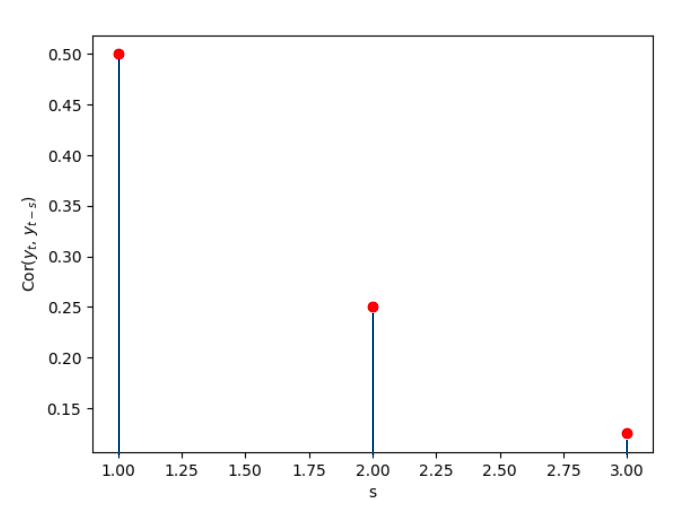
\includegraphics[scale=0.40]{corr.png}
    \caption{Correlogram Plot}
    \label{fig:my_label}
\end{figure}

\newpage

\textbf{c.} New process is given as 

\begin{equation}
    z_t = \frac{1}{\sqrt{2}}y_{1t} + \frac{1}{\sqrt{4}}y_{2t}
\end{equation}

One can find derive that E($y_{1t}$) = E($y_{2t}$) = 0 and Var($y_{1t}$) = Var($y_{2t}$) = 1 by following the same derivations in part (a) since the models are same in both questions. 
\\

\underline{Mean of $z_t$:}

\begin{align}
    \begin{split}
         E(z_t) = E(\frac{1}{\sqrt{2}}y_{1t} + \frac{1}{\sqrt{4}}y_{2t}) = \frac{1}{\sqrt{2}} E(y_{1t}) + \frac{1}{\sqrt{4}} E(y_{2t}) \\
         = \frac{1}{\sqrt{2}}*0 + \frac{1}{\sqrt{4}}*0 = 0
    \end{split}
\end{align}
\\

\underline{Variance of $z_t$:}

\begin{align}
    \begin{split}
        Var(z_t) = Var(\frac{1}{\sqrt{2}}y_{1t} + \frac{1}{\sqrt{4}}y_{2t}) = \frac{1}{2}Var(y_{1t}) + \frac{1}{4}Var(y_{2t}) \\
        \frac{1}{2}*1 + \frac{1}{4}*1 = \frac{3}{4}
    \end{split} 
\end{align}

\section{}

Models are given as following:

\begin{align}
    \begin{split}
        &(1) \ \ \ Y_t = \alpha X_t + u_{t1}, \ \  t=1,...,10  \ \ \ \  \sum {X_t}^2 = 4 \\
        &(2) \ \ \ Y_t = \beta X_t + u_{t2}, \ \  t=11,...,20  \ \ \ \  \sum {X_t}^2 = 4 \\
        &(3) \ \ \ Y_t = \gamma X_t + u_{t3}, \ \  t=1,...,20  
    \end{split}
\end{align}
\\

\underline{Model 1:} Given as in the question, this model exhibits
\begin{itemize}
    \item E($u_{t1}$) = 0  --- mean of error is zero
    \item E($u_{t1}$, $u_{s1}$) = 0  ---  no autocorrelation: correlation between error terms (where t $\neq$ s) is equal to 0
    \item E(${u_{t1}}^2$) = 2 --- no heterocedasticity: variance is constant for all observations 
\end{itemize}

Model (1) satisfies the Gauss-Markov Assumptions.
Therefore, Ordinary Least Squares estimator of the parameter is BLUE which is given in the question as $\hat{\alpha}_{OLS}$ = 0.8. 

\newpage

\underline{Model 2:} Given as in the question, this model exhibits
\begin{itemize}
    \item E($u_{t2}$) = 0  --- mean of error is zero
    \item E($u_{t2}$, $u_{s2}$) = 0  ---  no autocorrelation: correlation between error terms (where t $\neq$ s) is equal to 0
    \item E(${u_{t2}}^2$) = 4 --- no heterocedasticity: variance is constant for all observations 
\end{itemize}

Like Model (1), Model (2) also satisfies the Gauss-Markov Assumptions. Therefore, again OLS estimators will be BLUE which indicates that BLU estimator of $\beta$ is 1.6, as given in the question.
\\

\underline{Model 3:} Given as in the question, this model exhibits
\begin{itemize}
    \item E($u_{t3}$) = 0  --- mean of error is zero
    \item E($u_{t3}$, $u_{s3}$) = 0  ---  no autocorrelation: correlation between error terms (where t $\neq$ s) is equal to 0 (since E($u_{t1},u_{t2}$) = 0) 
    \item E(${u_{t1}}^2$) = 2 for t = 1,...,10 and E(${u_{t2}}^2$) = 4 for t = 11,...,20 --- heterocedasticity
\end{itemize}

Model (3) does not contain autocorrelation, but there is heterocedasticity in the model since variance is not constant for all observations. Under heterocedasticity, OLS estimators are not BLUE anymore. We need to use GLS, since we know the form of the heterocedasticity.
\\

Let's say ${\sigma_t}^2$ = ${\sigma}^2 \lambda_t$ where ${\sigma}^2$ = 4 and 

\begin{align}
    \begin{split}
        \lambda_t = \frac{1}{2} \ \ \ \ \text{for t = 1,...,10} \\
        \lambda_t = 1 \ \ \ \ \text{for t = 11,...,20}
    \end{split}
\end{align}

As a result,

\begin{align}
    \begin{split}
        & Var(u_t) = \sigma^2 * \lambda_t = 4 * \lambda_t \\
        & \frac{1}{\lambda_t}Var(u_t) = \sigma^2 = 4 \\
        & Var(\frac{1}{\sqrt{\lambda_t}}u_t) = \sigma^2 = 4
    \end{split}
\end{align}

Therefore, our weight is  $w_t = \frac{1}{\sqrt{\lambda_t}}$. Since, we have the weights for observations we can find the BLU estimator of $\gamma$ through OLS estimates since the model has no intercept term:

\begin{align}
    \begin{split}
        & \frac{\sum_{t=1}^{10} X_t Y_t}{\sum_{t=1}^{10} X_t^2} = \frac{\sum_{t=1}^{10} X_t Y_t}{4} = 0.8 \\ 
        & \sum_{t=1}^{10} X_t Y_t = 3.2 
    \end{split}
\end{align}

In the same way,

\begin{align}
    \begin{split}
         & \frac{\sum_{t=11}^{20} X_t Y_t}{\sum_{t=11}^{20} X_t^2} = \frac{\sum_{t=11}^{20} X_t Y_t}{4} = 1.6 \\
         & \sum_{t=11}^{20} X_t Y_t = 6.4
    \end{split}
\end{align}

Now we know the value of $\sum X_t Y_t$, we can find the GLS estimator of $\gamma$.

\begin{align}
    \begin{split}
        & \hat{\gamma} = \frac{\sum_{t=1}^{20} w_t^2 X_t Y_t}{\sum_{t=1}^{20} w_t^2 X_t^2} = \frac{2\sum_{t=1}^{10} X_t Y_t + 1\sum_{t=11}^{20} X_t Y_t}{2\sum_{t=1}^{10}X_t^2 + {1\sum_{t=11}^{20}X_t^2}} = \frac{2*3.2 + 1*6.4}{2*4 + 1*4} = 1.06
    \end{split}
\end{align}
\\

GLS estimator, Best Linear Unbiased Estimator, of $\gamma$ is equal to 1.06.
\\

\textbf{c.}

Estimated variance of GLS estimator of $\gamma$:

\begin{align}
    \begin{split}
        & Var(\hat{\gamma}) = \frac{\sigma^2}{\sum_{t=1}^{20} w_t^2 X_t^2} = \frac{\sigma^2}{2\sum_{t=1}^{10}X_t^2 + {1\sum_{t=11}^{20}X_t^2}} = \frac{4}{2*4 + 1*4} = 0.33
    \end{split}
\end{align}
\\

To discuss the efficiency, we need to compare GLS estimate to OLS estimate. Let's first find the OLS estimate of $\gamma$:

\begin{align}
    \begin{split}
        \Tilde{\gamma} = \frac{\sum_{t=1}^{20} X_t Y_t}{\sum_{t=1}^{20} X_t^2} = \frac{3.2 + 6.4}{4 + 4} = 1.2
    \end{split}
\end{align}

Error variance in OLS model:

\begin{align}
    \begin{split}
        \sigma^2_{OLS} = E(u_t^2) = \frac{\sum u_t^2}{20} = \frac{20 + 40}{20} = 3
    \end{split}
\end{align}

Variance of OLS estimator $\Tilde{\gamma}$:

\begin{equation}
    Var(\Tilde{\gamma}) = \frac{\sigma^2_{OLS}}{\sum X_t^2} = \frac{3}{4 + 4} = 0.375
\end{equation}

One can easily notice that,

\begin{equation}
    Var(\hat{\gamma}_{GLS}) = 0.33 < 0.375 = Var(\Tilde{\gamma}_{OLS})
\end{equation}

Since the variance of GLS estimator of $\gamma$ is smaller, it is more efficient than the OLS estimator of $\gamma$.


\newpage

\Large
\underline{\textbf{Part B}}
\small

\setcounter{section}{1}

\section{}

\textbf{a.}

\underline{Model 1:}

\begin{itemize}
    \item Expected change in consumption on life insurance is equal to 1.37 per unit change in disposable income while cost of life insurance held constant.
    \item Expected change in consumption on life insurance is equal to -0.6 per unit change in real cost of life insurance while disposable income held constant.
    \item $R^2$ is equal to 0.958, which means 96 percent of the variability in consumption on life insurance can be explained by the variations in disposable income and cost of life insurance.
    \item Durbin-Watson test statistic is equal to 0.36 which is smaller than 2. Therefore, it shows a positive autocorrelation in the model.
\end{itemize}


\underline{Model 2:}

\begin{itemize}
     \item Expected change in consumption on life insurance is equal to 1.41 per unit change in disposable income while cost of life insurance held constant.
    \item Expected change in consumption on life insurance is equal to -0.75 per unit change in real cost of life insurance while disposable income held constant.
    \item $R^2$ is equal to 0.985, which means 98.5 percent of the variability in consumption on life insurance can be explained by the variations in disposable income and cost of life insurance.
    \item Durbin-Watson test statistic is equal to 1.90 which is very close to 2. Therefore, we can say that there is no autocorrelation in the Model (2).
\end{itemize}

One can show that there is no autocorrelation in Model (2) by looking at the figure below. 

\begin{figure}[h]
    \centering
    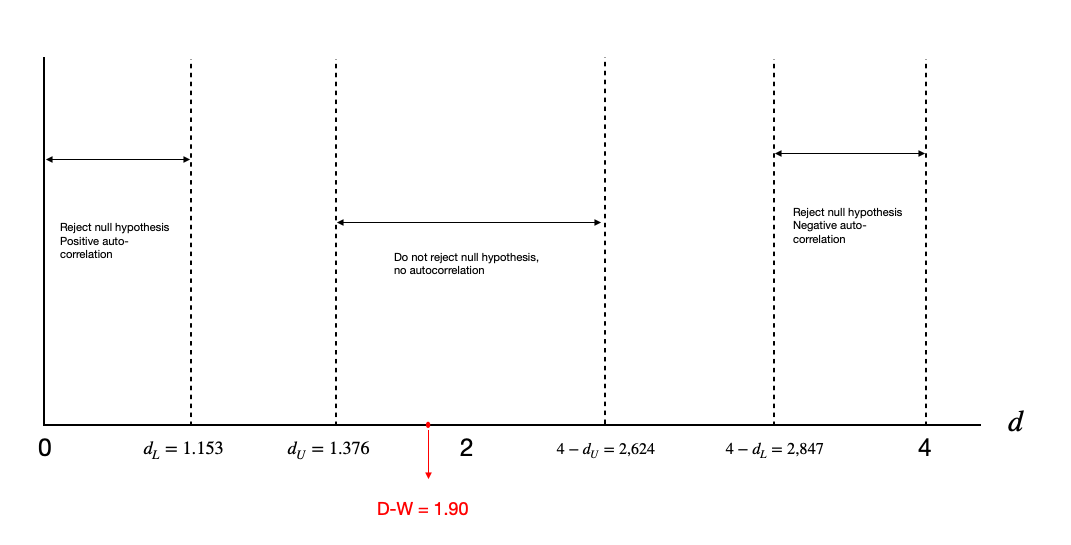
\includegraphics[scale=0.3]{D-W Figure.png}
\end{figure}

Since our test statistic does not fall into the rejection region, we fail to reject the null hypothesis and conclude that there is no autocorrelation in the Model (2).

\newpage

\underline{Conclusion:} Model (1) uses the OLS method where Model (2) uses the C-O estimation. It is obvious from D-W statistic that there is autocorrelation in Model (1) which makes the OLS estimates inefficient and they are no longer best linear unbiased estimators. However, using C-O estimation we can avoid the problem of autocorrelation which is proven by the D-W test statistic in Model (2). In conclusion, Model (2) is better because there is no autocorrelation in the model.
\\



\textbf{b.} If I would have to choose between Model (1)-(4), I would choose Model (2) for several reasons:

\begin{itemize}
    \item D-W statistic in Model (2) is 1.90 which is very close to 2 so indicates no autocorrelation. In this context, Model (1) is not appropiate because D-W statistic is very far from 2 which indicates autocorrelation in the model. Remaining models (3) and (4) have also D-W statistic close to 2, however, the equations include a lagged dependent variable as an explanatory variable (ie. $cr_{t-1}$). Thus, D-W statistics are not valid. We cannot say that there is no autocorrelation according to D-W test. 
    \item Model(3) has a little larger $R^2$ value than Model (2) but it also has more explanatory variables so comparing $R^2$ values can be misleading. Moreover, standard errors of coefficient estimates in Model (3) is larger than in the Model (2) which is a bad thing because it lowers the accuracy of the estimates. Therefore, at this step I wouldn't choose Model (3) and keep using Model (2).
    \item Even though Model (4) has smaller standard errors of coefficient estimates compared to Model (2), I would still stick with Model (2) because in Model (4), estimated coefficient of the parameters are very close to 0 which nearly indicates that the covariates do not have any significant importance on the dependent variable. We can easily show the significance of the model parameters with using t-test:
\end{itemize}

\underline{For $yd_t$:} $H_0$ = coefficient of $yd_t$: $\beta_1$ = 0 vs. $H_a$ = coefficient of $yd_t$: $\beta_1 \neq$ 0

\begin{equation}
    t_{stat} = \frac{\hat{\beta_1} - \beta_1 }{se(\hat{\beta_1})} =  \frac{0.28 - 0 }{0.20} = 1.4 < 1.694 = t_{0.05,32}
\end{equation}

We fail to reject the null hypothesis and conclude that disposable income does not have any significant importance on consumption on life insurance while cost of life insurance and consumption on life insurance(at time t-1) are in the model.
\\

\underline{For $ic_t$:} $H_0$ = coefficient of $ic_t$: $\beta_2$ = 0 vs. $H_a$ = coefficient of $ic_t$: $\beta_2 \neq$ 0

\begin{equation}
    t_{stat} = \frac{\hat{\beta_2} - \beta_2 }{se(\hat{\beta_2})} =  \frac{-0.26 - 0 }{0.21} = - 1.23 > -1.694 = -t_{0.05,32}
\end{equation}

Again, we fail to reject the null hypothesis and conclude that cost of life insurance does not have any significant importance on consumption on life insurance while disposable income and consumption on life insurance(at time t-1) are in the model.
\\

However, these two variables were significant in Model (1) and (2) when $cr_{t-1}$ was not in the model. Maybe, adding $cr_{t-1}$ to the model created multicollinearity in the model. Going from Model (1) to (4), researcher probably suspected autocorrelation and decided to add $cr_{t-1}$ so that model can avoid autocorrelation problem. However, still there might be autocorrelation caused by a structural break or an omitted variable and we cannot test the model through D-W statistic because it is invalid due to lag variable in the Model (4). Since the autocorrelation problem is solved for sure in Model (2), I would choose Model (2) instead of Model (4).
\\

\underline{Conclusion:} I think the most appropiate model among (1)-(4) is Model (2) because it does not contain autocorrelation, its coefficient estimates are large enough to indicate a significant statistical relationship in the model and they have small standard errors, and finally it has a large $R^2$ which is 0.985.
\\

\newpage

\textbf{c.}
\\

I don't think that commentor's model specification is appropiate. We have already discovered that disposable income and cost of insurance have significant importance on consumption on insurance in Model (2). Also, Model (5) predicts the value of dependent variable only by looking its previous value and a constant term. Therefore, it indicates a random walk with drift which is usually used in default expectation such as real GDP data. Researcher should apply Dickey-Fuller Test to the data to check if exhibits a random walk with drift. I don't think the context in this question fits to the random walk with drift. In fact, the intercept term is positive which means the consumption on life insurance increases over time. However, as it is shown in all other models, when real cost of insurance increase, consumption of life insurance decreases. So, it cannot be always upward sloped. I think consumption on life insurance depends on both disposable income and cost of life insurance.  As a result, these variables should not be omitted and it is better to omit the $cr_{t-1}$ from the model. Therefore, again using Model (2) makes more sense for me.  
\\

\underline{Model 5:}

\begin{itemize}
    \item Expected change in consumption on life insurance(at time t) is 0.98 per unit change in consumption on life insurance(at time t-1).
    \item 98.5 percent of variations in consumption on life insurance(at time t) can be explain by the variations in consumption on life insurance(at time t-1)
     \item D-W statistic is very close to 2, but it is invalid due to the existence of dependent variable lag. Autocorrelation may still exist. 
\end{itemize}











    




 

\end{document}


